%!TeX program = xelatex
%Do not change
\documentclass[12pt, oneside]{article}
\usepackage{amssymb,amsmath}
\usepackage[margin=1in]{geometry}
\usepackage{textpos}
\usepackage{float}
\usepackage{booktabs}
%\usepackage{color}
\usepackage{graphicx}
\usepackage[inter-unit-product =\cdot]{siunitx}
\let\DeclareUSUnit\DeclareSIUnit
\let\US\SI
\DeclareUSUnit\inch{in}
\DeclareUSUnit\foot{ft}
\DeclareUSUnit\mile{mi}
\DeclareUSUnit\foot{ft}
\DeclareUSUnit\slug{slug}
\DeclareUSUnit\pound{lb}
\DeclareUSUnit\psi{psi}
\DeclareUSUnit\Msi{Msi}
\DeclareUSUnit\ksi{ksi}

\usepackage{tikz}
\usetikzlibrary{positioning}
%\usepackage{tikz-3dplot}
\usepackage{pgfopts}
%\usepackage{wasysym}
\usepackage{stanli}

% You may add the packages you need here
\begin{document}

%TODO change numbers in problems
\begin{textblock*}{4cm}(-1.7cm,-2.3cm)
\noindent {\scriptsize AE333 Fall 2020}
\end{textblock*}

%Do not modify other than putting your name where stated
\begin{textblock*}{8cm}(12.5cm,-1cm)
\noindent {Name: }
\end{textblock*}
%Do not modify other than typing your acknowledgement where stated
\begin{textblock*}{13.5cm}(-1.7cm,-1.8cm)
%\noindent \textit{\footnotesize Acknowledgement: Your acknowledgement for collaboration and other sources goes here. }
\end{textblock*}

\vspace{1cm}

%Do not modify other than typing the homework number after #
\begin{center}
\textbf{\Large Homework 10}

\textbf{Due 10 November 2020}
\end{center}

\begin{enumerate}
	\item %12-99
		Find the reactions at each support, assume $EI$ is constant and neglect axial load.
		\begin{figure}[H]
			\centering
			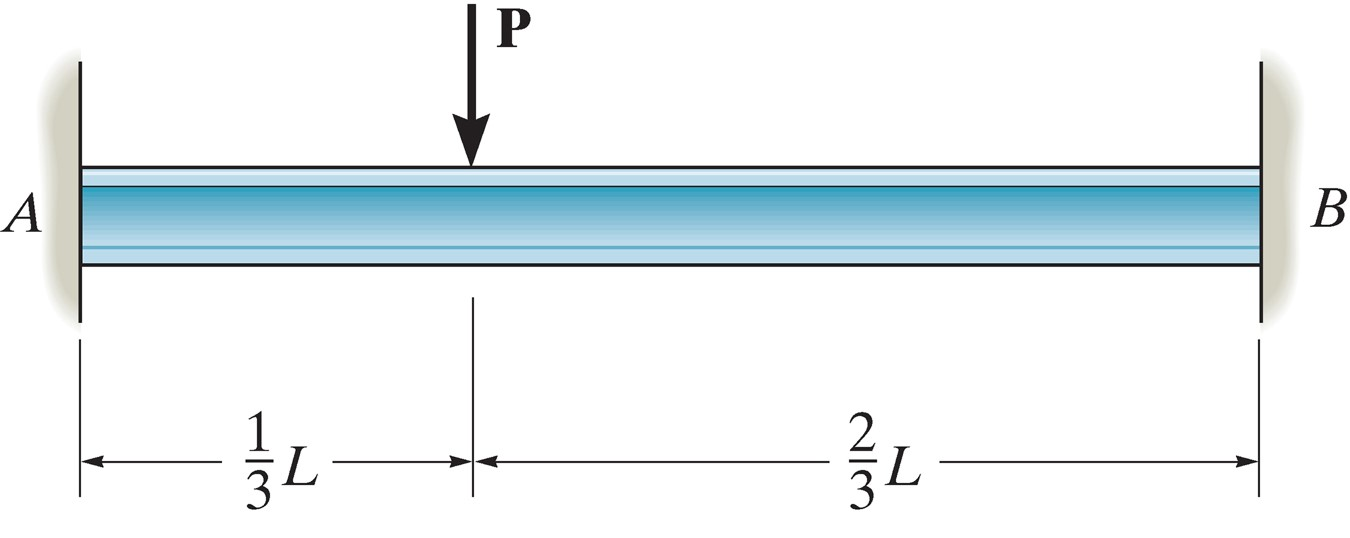
\includegraphics[width=0.6\linewidth]{12-99}
		\end{figure}

	\item %12-106
		Find the maximum deflection in terms of some constant $EI$
		\begin{figure}[H]
			\centering
			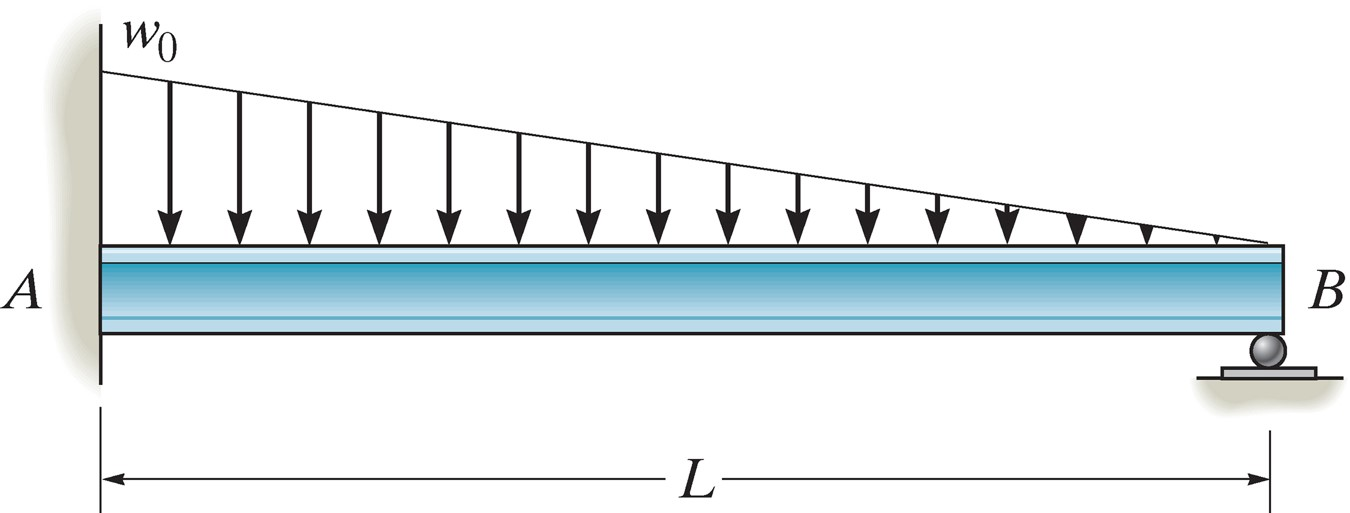
\includegraphics[width=0.6\linewidth]{12-106}
		\end{figure}

	\item %12-107
		Find the maximum deflection in terms of some constant $EI$
		\begin{figure}[H]
			\centering
			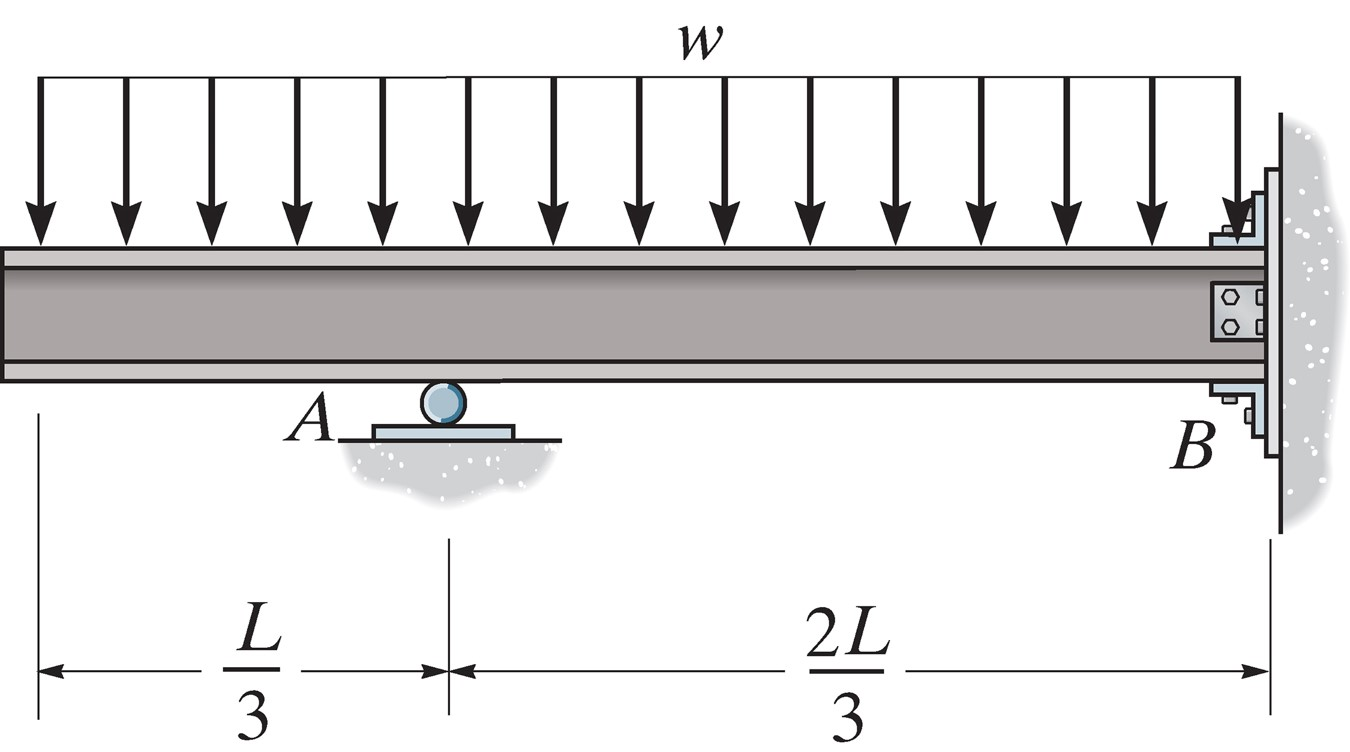
\includegraphics[width=0.6\linewidth]{12-107}
		\end{figure}
		\newpage

	\item %12-121
		Find the reactions at each of the supports, assuming $A$ is a fixed support and $B$ is a roller.
		\begin{figure}[H]
			\centering
			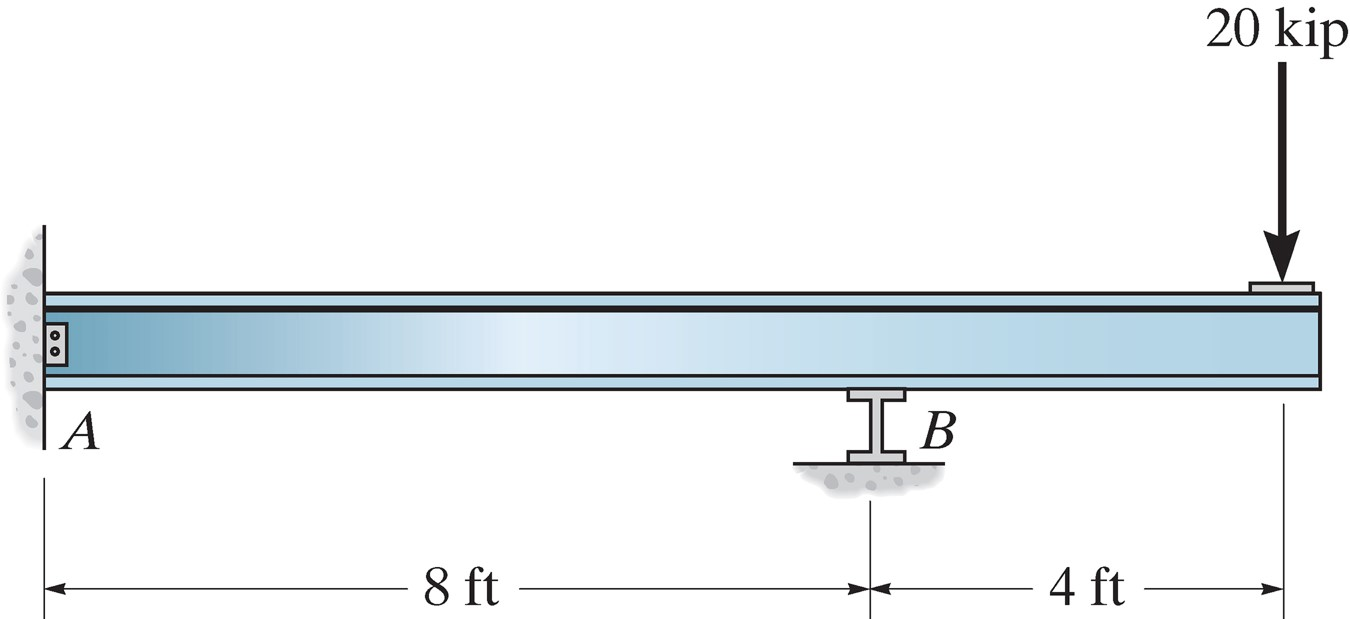
\includegraphics[width=0.6\linewidth]{12-121}
		\end{figure}

	\item 
		Dr. Smith has decided to add an extra support at the center of his daughter's bed he is building.
		Compare the maximum deflection with and without the support assuming that the piece in question can be modeled as shown below.
		Note that the beam is 6 feet long with a support added exactly in the middle and his daughter weighs 30 pounds, neglect any horizontal reaction forces.
		Assume the beam is a solid rectangle made from pine 1.5 inches thick and 3 inches tall.
		\begin{figure}[htpb]
		\begin{center}
		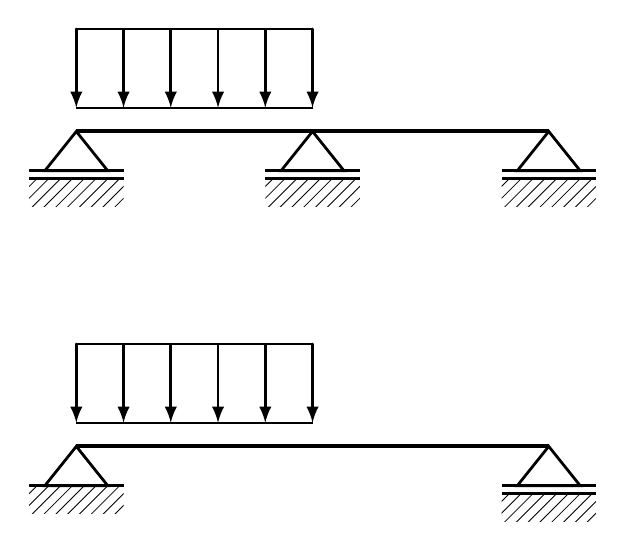
\begin{tikzpicture}
			\point{a}{0}{0};
			\point{b}{6}{0};
			\point{c}{0}{4};
			\point{d}{3}{4};
			\point{e}{6}{4};
			\point{f}{3}{0};
			\beam{2}{a}{b};
			\beam{2}{c}{e};
			\support{1}{a};
			\support{2}{b};
			\support{2}{c};
			\support{2}{d};
			\support{2}{e};
			\lineload{1}{a}{f};
			\lineload{1}{c}{d};
		\end{tikzpicture}
		\end{center}
		\end{figure}

\end{enumerate}
\end{document}
